\colorformatcornflowerblue

\begin{document}

% -------------------------------------------------------------------------------
% -------------------------------------------------------------------------------

\begin{frame}[plain]
  
\titlepage

\begin{center}

\includegraphics[scale=0.45]{unine}
\end{center}

\end{frame}

% -------------------------------------------------------------------------------
% -------------------------------------------------------------------------------

\subtitle[Introduction]{Introduction}

\begin{frame}{Erasure coding}
    \todo[inline]{Recap about what is erasure coding}
\end{frame}

\begin{frame}{Motivation}
    \todo[inline]{Why we created \sys}
\end{frame}

\subtitle[Architecture]{Architecture}

\begin{frame}{Technical components}
    \centering
    % TikZ figure showing the relations between all components of the erasure codes tester

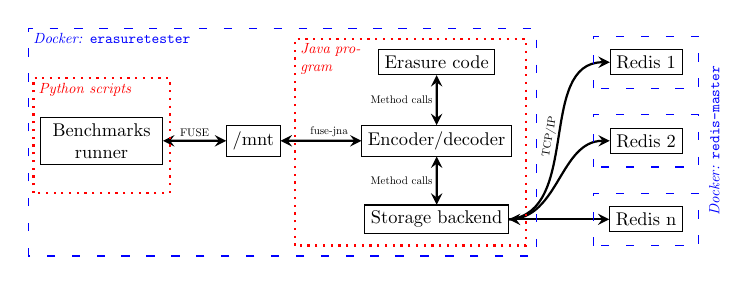
\begin{tikzpicture}[transform shape,scale=0.665]
\node[draw, text width=2.1cm, text centered] (bench) at (2.6, 1.5) {Benchmarks runner};
\node[draw] (dir) at (5.5, 1.5) {/mnt};
\node[draw] (fed) at (9, 1.5) {Encoder/decoder};
\node[draw] (sb) at (9, 0) {Storage backend};
\node[draw] (ec) at (9, 3) {Erasure code};
\node[draw] (r1) at (13, 3) {Redis 1};
\node[draw] (r2) at (13, 1.5) {Redis 2};
\node[draw] (r3) at (13, 0) {Redis n};

\draw[<->,thick,>=stealth] (bench) -- (dir) node[midway,above,scale=0.6]{FUSE};
\draw[<->,thick,>=stealth] (dir) -- (fed) node[pos=0.6,above,scale=0.6]{fuse-jna};
\draw[<->,thick,>=stealth] (fed) -- (ec)
node[pos=0.5,left,scale=0.6]{Method calls};
\draw[<->,thick,>=stealth] (fed) -- (sb)
node[pos=0.5,left,scale=0.6]{Method calls};
\draw[->,thick,>=stealth] (sb.east) to[out=5,in=180] node[sloped,midway,scale=0.6,above]{TCP/IP} (r1.west);
\draw[->,thick,>=stealth,out=0,in=180] (sb.east) to[out=0,in=180] (r2.west);
\draw[<->,thick,>=stealth] (sb.east) -- (r3.west);

\draw[loosely dashed,blue] (1.2,-0.7) rectangle (10.9,3.65);
\draw[loosely dashed,blue] (12,2.5) rectangle (14,3.5);
\draw[loosely dashed,blue] (12,1) rectangle (14,2);
\draw[loosely dashed,blue] (12,-0.5) rectangle (14,0.5);
\draw[dotted,red,thick] (6.3,-0.5) rectangle (10.7,3.45);
\draw[dotted,red,thick] (1.3,0.5) rectangle (3.9,2.7);

\draw (6.3,3.45) node[below right,red,scale=0.8, text width=1.5cm] {\textit{Java program}};
\draw (1.3,2.7) node[below right,red,scale=0.8] {\textit{Python scripts}};
\draw (1.2,3.65) node[below right,blue,scale=0.8] {\textit{Docker:} \texttt{erasuretester}};
\draw (14.3,1.5) node[blue,scale=0.8,rotate=90] {\textit{Docker:} \texttt{redis-master}};
\end{tikzpicture}

\end{frame}

\begin{frame}{Key features of \sys}
    \begin{itemize}
        \item Possible to run existing benchmarks
        \item Automated benchmarks execution
        \item Can run on heterogeneous nodes, as long as Docker Swarm is supported
    \end{itemize}
\end{frame}

\subtitle[Evaluation]{Evaluation}

\begin{frame}{Evaluation}
    \todo[inline]{Present some interesting results}
\end{frame}

\subtitle[Conclusion]{Conclusion}

\begin{frame}{Conclusion}
    \begin{itemize}
        \item Things
    \end{itemize}
\end{frame}

% -------------------------------------------------------------------------------
% -------------------------------------------------------------------------------

\end{document}

% -------------------------------------------------------------------------------
